\begin{boxedabstract}

The recent success of large language models (LLMs) has renewed interest in whether recommender systems can achieve similar scaling benefits. Conventional recommenders, dominated by massive embedding tables, tend to plateau as embedding dimensions grow. In contrast, the emerging generative paradigm replaces embeddings with compact Semantic ID (SID) sequences produced by autoregressive Transformers. Yet most industrial deployments remain proprietary, leaving two fundamental questions open: (1) Do the expected scaling laws hold on public benchmarks? (2) What is the minimal post-training recipe that enables competitive performance?

We present \textbf{MiniOneRec}, to the best of our knowledge, the first fully open-source generative recommendation framework, which provides an end-to-end workflow spanning SID construction, supervised fine-tuning, and recommendation-oriented reinforcement learning. We generate SIDs via a Residual Quantized VAE and post-train Qwen backbones ranging from 0.5B to 7B parameters on the Amazon Review dataset. Our experiments reveal a consistent downward trend in both training and evaluation losses with increasing model size, validating the parameter efficiency of the generative approach. To further enhance performance, we propose a lightweight yet effective post-training pipeline that (1) enforces full-process SID alignment and (2) applies reinforcement learning with constrained decoding and hybrid rewards. Together, these techniques yield significant improvements in both ranking accuracy and candidate diversity.
% Our codes are available at 

\faGithub\ \url{https://github.com/AkaliKong/MiniOneRec}

\hspace{-0.3em} \raisebox{-0.2em}{
\includegraphics[height=0.9em]{figures/hf-logo.png}}
\url{https://huggingface.co/kkknight/MiniOneRec}


\end{boxedabstract}

%\begin{center}
%  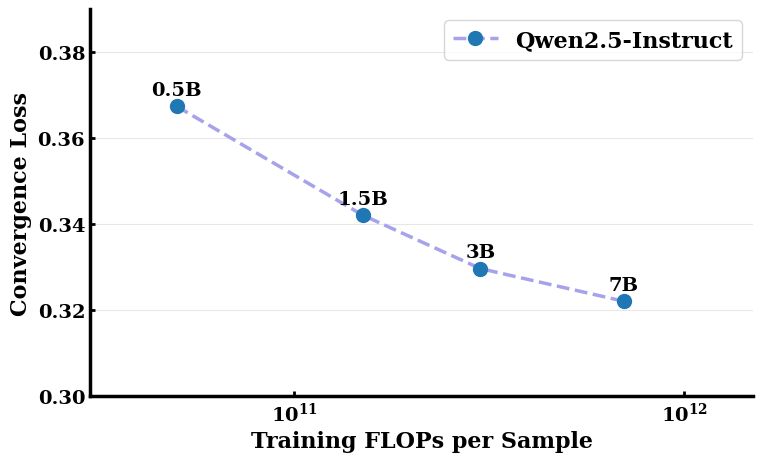
\includegraphics[width=0.66\textwidth]{figures/scaling.png}
%  \captionsetup{type=figure}       
%  \captionof{figure}{Scaling curves from 0.5B to 7B parameters.}
%  \label{fig:scaling}
%\end{center}
% \end{abstract}

\begin{center}
\begin{minipage}[t]{0.46\textwidth}
\centering
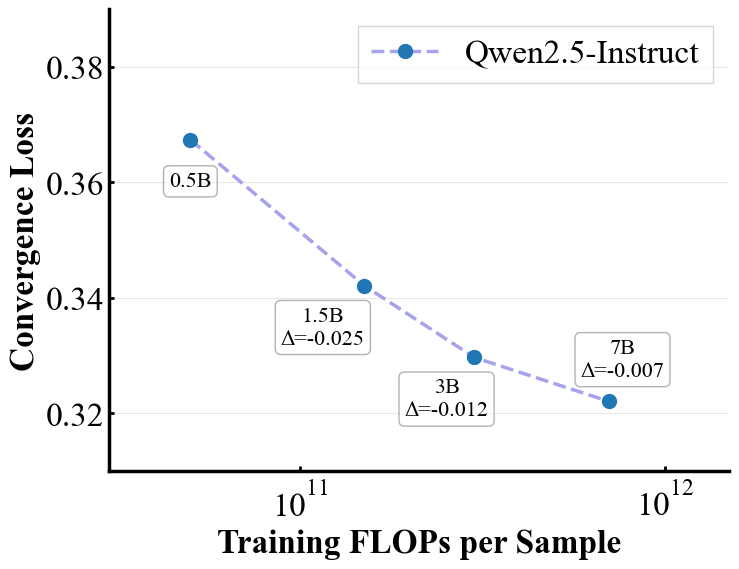
\includegraphics[width=\linewidth]{figures/scaling_big.png}
\end{minipage}\hfill
\begin{minipage}[t]{0.46\textwidth}
\centering
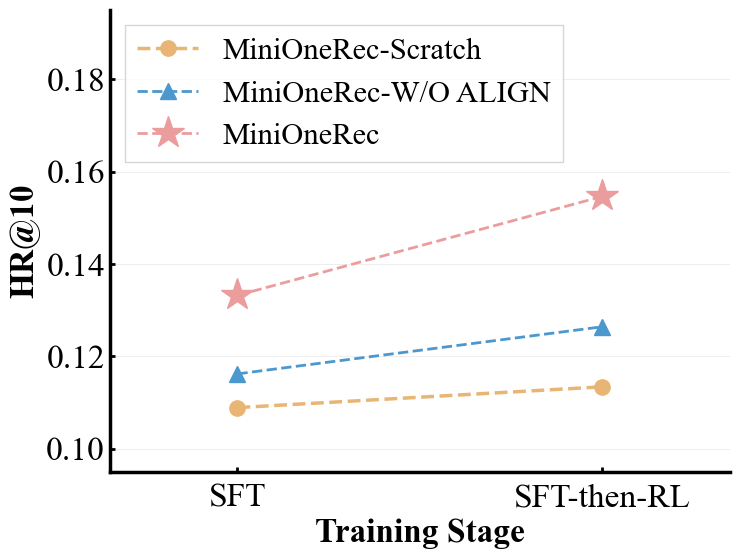
\includegraphics[width=\linewidth]{figures/llmmatter_big.png}
\end{minipage}
\captionsetup{type=figure}
\captionof{figure}{Left: Scaling curves from 0.5B to 7B parameters. Right: Effect of world knowledge on model performance: MiniOneRec-W/O ALIGN uses pretrained LLM weights but omits SID–text alignment, while MiniOneRec-Scratch is trained from random initialization and omits alignment.}
\label{fig:scaling}
\end{center}
